% All the result and analysis
\chapter{The Results}

\begin{quote}
\textsl{``The most incomprehensible thing about the world is that it is comprehensible." - Albert Einstein}
\end{quote}

\section{Introduction}
It is always a challenge to extract and analyze data from an Artificial Life simulation. Data and analysis in this simulation has been concentrated on evaluating whether evolution of mimicry has taken place. This evaluation can be made with the number of different rings that has been created and the size of each of those rings along with the population of palatable and unpalatable species. Also it can be established whether Batesian Mimicry and Mullerian Mimicry has taken effect by analyzing the data set of these populations.

\section{Mimicry Ring Reports}
The mimicry ring reports consists entirely of the population of prey species categorized according to patterns and palatability. Data is stored at every instance of time of the simulation keeping an interval of 10 iterations. As the number of rings that get generated reaches as many as 50 or more, and all the population of ring do not last for the entire simulation, so while storing data we have taken the most populous of the surviving 8 rings to plot. Parameters are mentioned in Table \ref{tab:ring-report-control-parameters}.

\begin{table}[H]
\centering
\begin{tabular}{| p{2cm} | >{\centering} p{2.2cm} | p{8cm} |}
	\hline
		\textbf{Parameter} & \textbf{Value} & \textbf{Description} \\ \hline
		Mimicry Ring Hamming Distance & 10 \% of the Pattern Size & If the Hamming distance between the pattern of the model and the mimic is 10 \% the size of the pattern then they are considered within the same ring.\\ \hline
		Number of Rings to report & 8 & This value is the number of most populous rings that are included in the report.\\
	\hline
\end{tabular}
\caption{Parameters to mimicry ring report.}
\label{tab:ring-report-control-parameters}
\end{table}

\section{Initial configuration with two prey species}
% Put the table here
\begin{table}[H]
\centering
\begin{tabular}{|l|l|c|c|l|c|}
  \hline
   														&\multicolumn{3}{|c|}{Prey configuration} 																	
   														& \multicolumn{2}{|c|}{Predator configuration} \\ \hline
  \multirow{2}{*}{Population} & Rule110 (Palatable) & \parbox[c]{2.1em}{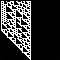
\includegraphics[scale=0.50]{images/CARule110}} & 108 
  														& \multicolumn{2}{|c|}{\multirow{2}{*}{10}} \\ \cline{2-4}
  					 									& Rule30 (Unpalatable)& \parbox[c]{2.1em}{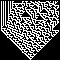
\includegraphics[scale=0.50]{images/CARule30}}  & 108 
  					 									& \multicolumn{2}{|c|}{}\\ \hline
  \multirow{2}{*}{Reproduction} & Age Limit & \multicolumn{2}{|c|}{100}  & \multicolumn{2}{|c|}{500} \\ \cline{2-6}
  						 									& Interval  & \multicolumn{2}{|c|}{1000} & \multicolumn{2}{|c|}{1000} \\ \hline
  \multirow{2}{*}{Mutation Rate} & Pattern   & \multicolumn{2}{|c|}{0.05} & \multicolumn{2}{|c|}{\multirow{2}{*}{0.03}} \\ \cline{2-4}
  						 									 & Genome    & \multicolumn{2}{|c|}{0.5}  & \multicolumn{2}{|c|}{} \\ \hline
  Demise Age	 									 & \multicolumn{3}{|c|}{2000}							& \multicolumn{2}{|c|}{2500} \\ \hline
  Minimum Attack Age						 & \multicolumn{3}{|c|}{} 						    & \multicolumn{2}{|c|}{500} \\ \hline
  \multirow{2}{*}{Memory Configuration} & \multicolumn{3}{|c|}{} 					& Minimum & 2 \\ \cline{5-6}
   																			& \multicolumn{3}{|c|}{} 					& Maximum & 10 \\ \hline  
\end{tabular}
\caption{Agent configuration of 2 prey species}
\label{tab:config-table-2-prey}
\end{table}

The set of parameters in Table \ref{tab:config-table-2-prey} were carefully selected to be the initial condition for this run of the simulation. This test has been done with two sets of prey species with very different CA pattern and with opposite palatability and equal population. To control reproduction of the prey species their age limit has been set to 100 iterations into the time the species were alive. And the reproduction interval was set to 1000 iterations.

Pattern mutation rate has been set to a minimal level of 0.05 as by increasing this variable it is possible to increase the size of the number of mimicry rings present in the simulation. The Genome mutation rate controls the rate at which genome of the child prey species will deviate from their parents. As mentioned earlier the genome mutation rate has been separated from the pattern mutation rate to bring more control to the number of mimicry rings generated.

Prey demise age has been kept to 2000 iterations while predator demise age is set to 2500. But later in the following results predator demise age has been increased to 5000 iterations. Predators in this simulation generates selection pressure for the evolution of mimicry. So the longer a predator is present in the simulation it will be making intelligent decisions in term of selecting which prey species to consume and which one to avoid. But with the current rate of demise for predator we were able to create successful mimetic population of prey species as we will see in the analysis in the following results.

Initial population of predator species has been set to 10 which is in accordance with the prey population in the simulation. The reason for such low number of predator is, unlike prey species which are consumed by predators, there is no cause for the predator species to die accept their natural cause of death, that is to reach their demise age. So predator population can explode very easily. That is why their population is controlled in a restrictive manner with the help of high reproduction age limit and reproduction age interval.

The memory configuration size for predators is a very interesting parameter. The minimum memory size is directly associated with the number of prey species with which we initiate the simulation. Otherwise evolution of mimicry is not observed. As mentioned in Table \ref{tab:predator-control-parameters} the minimum memory size is the number of prey species predator would consume before starting to make decisive consumption of prey species. After the initial birth of a predator and when the minimum attack age is crossed, it starts consuming prey species present in its vicinity without making any judgment. At this point its memory size is zero. As long as the minimum memory size is not reached predators will blindly consume prey species and insert their CA pattern and associated palatability into its Hopfield memory bank. No later than the minimum memory size has been reached, predators will start making intelligent decision about consuming its prey species. When catching a prey if its memory tells that it is palatable, it will consume that prey. Otherwise if memory recognizes it to be unpalatable predator will certainly let it go.

Now as we know the behavior of Hopfield memory, a recognition result will always be achieved depending on the similarity of the patterns stored in memory. So when minimum memory size has been reached the predator will always make a decision based on the similarity of the prey pattern previously captured and the patterns stored in memory.

% Put the image
\begin{figure}[H]
	\centering
	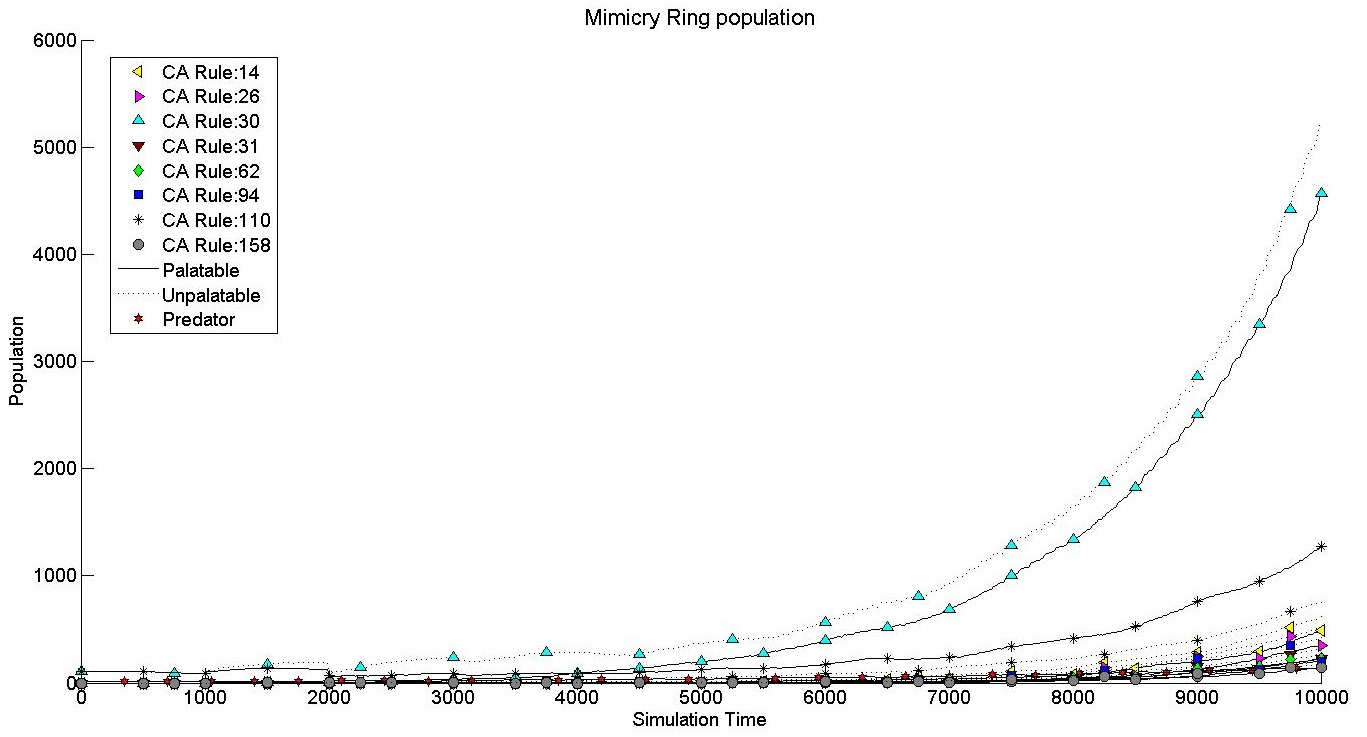
\includegraphics[scale=0.50]{images/simTime10k-2Prey}
	\caption[Population distribution of mimicry rings (2 prey species)]{Population distribution of mimicry rings, initialized with 2 prey species.}
	\label{fig:plot-2-prey}
\end{figure}

The plot in Figure \ref{fig:plot-2-prey} is simulation time verses prey population after running it for over 10000 iterations. With the initial configuration in the above table we can observe that multiple rings of prey population has been created. Two prey species are in a ring if their CA pattern have a hamming distance within 10 bits, parameter mentioned in Table \ref{tab:ring-report-control-parameters}. Population of palatable species has been represented with line curve while population of unpalatable species has been presented with dotted curve. Different signs of squares, triangles and diamonds have been used to distinguish between species of prey population. The simulation was initiated with two prey species having CA rule of 30 and 110 and being palatable and unpalatable consecutively.

By closely observing the graph we could see the population of two species have started dropping at around time 500 when the initial predator population reaches this maturity for consuming prey species. At around time 1000 the prey population starts reproducing as the population increases. At around the same time different other species of prey population gets to be born with mutated CA patterns. Over time the population of CA Rule 110 dominates the population as most predators recognizes it as unpalatable. And similarly a population of CA Rule 110 or within the same ring of palatable species starts rising, while at one point overlaps the population of CA Rule 30 (Time: 5000 approx.) which was initially considered as a set of palatable species.

We can observe from the above results that the evolution of mimicry has taken effect. A population of mimics were successfully able to exceed the population of other prey species the reason being avoidance by predators of prey pattern similar to unpalatable ones. We can conclude that Batesian mimicry has taken effect in the simulation.

The above configuration in Table \ref{tab:config-table-2-prey} is also the most appropriate condition for Mullerian Mimicry. We can observe that a single pattern of unpalatable species dominate the entire population. These effects can be observed in this configuration where we can see the continuous increment of prey and predator population and eventually behaviors of Mullerian mimicry, where all prey species converge to a single ring of CA pattern.

%Put the number of rings picture:
\begin{figure}[H]
	\centering
	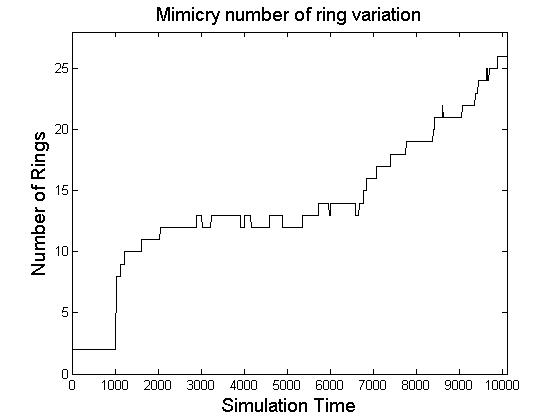
\includegraphics[scale=0.50]{images/ringSize10k-2Prey}
	\caption[Number of mimicry rings (2 prey species)]{Number of mimicry rings, initialized with 2 prey species.}
	\label{fig:ringSize10k-2Prey}
\end{figure}

As it can be observed from Figure \ref{fig:ringSize10k-2Prey} the number of rings in this simulation makes a slow increase from 2 at the initial configuration to 33 rings at the end of 10000 iterations. We can observe that a small change in CA genetic representation can have a very large effect in terms of the phenotype of the pattern with which the prey is represented. For example if we observe the set of pattern genotype with very different phenotype in Table \ref{tab:diff-in-pattern}.

%CARule table
\begin{table}[H]
\centering
\begin{tabular}{|l|c|c|c|}
  \hline
  CA Rule & \(60 \equiv 00111100\) & \(61 \equiv 00111101\) & \(62 \equiv 00111110 \) \\ \hline
  Pattern & \parbox[c]{2.1em}{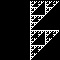
\includegraphics[scale=0.50]{images/CARule60}} 
  				& \parbox[c]{2.1em}{
\includegraphics[scale=0.50]{images/CARule61}} 
  				& \parbox[c]{2.1em}{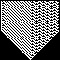
\includegraphics[scale=0.50]{images/CARule62}}\\
  \hline
\end{tabular}
\caption{Difference in prey pattern genotype and phenotype}
\label{tab:diff-in-pattern}
\end{table}

All the patterns in Table \ref{tab:diff-in-pattern} have a genetic bit difference of 1. So by a single mutation there can be three different set of phenotype for a child organism from its parent. This is largely the reason for the increased number of Rings created in the simulation. Only the 8 most populous rings have presented in the graph above with population verses simulation time.

%Screenshot of the simulation
\begin{figure}[H]
	\centering
	\label{fig:screenshot-simTime7600-2-prey}
	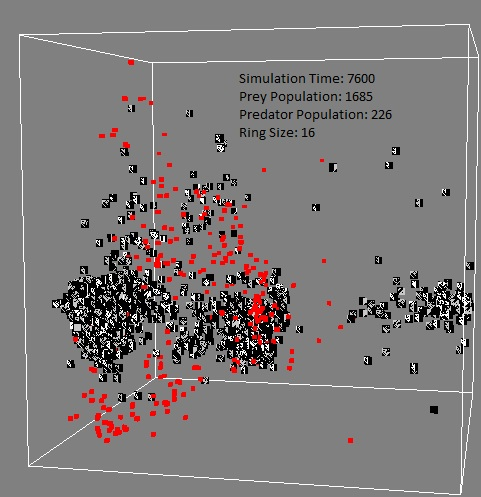
\includegraphics[scale=0.55]{images/simTime7600}
	\caption[Graphical representation of the model (simulation time: 7600)]{Graphical representation of the model, simulation time: 7600.}
\end{figure}

The screen shot in Figure \ref{fig:screenshot-simTime7600-2-prey} is for one instance of time of the simulation. The red agents are predators while the black agents with different textured patterns are the prey species. According to their behavior most of the prey species are flocking together in a group while also being chased by the predators, whose sole purpose is to consume prey species. 

\section{Initial configuration with four prey species}
\begin{table}[H]
\centering
\begin{tabular}{|l|l|c|c|l|c|}
  \hline
   														&\multicolumn{3}{|c|}{Prey configuration} 																	
   														& \multicolumn{2}{|c|}{Predator configuration} \\ \hline
  \multirow{4}{*}{Population} & Rule110 (Unpalatable) & \parbox[c]{2.1em}{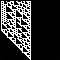
\includegraphics[scale=0.50]{images/CARule110}} 
  																										& 50 & \multicolumn{2}{|c|}{\multirow{4}{*}{10}} \\ \cline{2-4}
  					 									& Rule30 (Palatable)& \parbox[c]{2.1em}{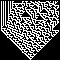
\includegraphics[scale=0.50]{images/CARule30}}
  					 																					& 50 & \multicolumn{2}{|c|}{}\\ \cline{2-4}
  					 									& Rule55 (Unpalatable)& \parbox[c]{2.1em}{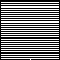
\includegraphics[scale=0.50]{images/CARule55}}
  					 																					& 50 & \multicolumn{2}{|c|}{}\\ \cline{2-4}
  					 									& Rule190 (Palatable)& \parbox[c]{2.1em}{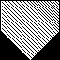
\includegraphics[scale=0.50]{images/CARule190}}
  					 																					& 50 & \multicolumn{2}{|c|}{}\\ \hline
  \multirow{2}{*}{Reproduction} & Age Limit & \multicolumn{2}{|c|}{100}  & \multicolumn{2}{|c|}{500} \\ \cline{2-6}
  						 									& Interval  & \multicolumn{2}{|c|}{1000} & \multicolumn{2}{|c|}{1400} \\ \hline
  \multirow{2}{*}{Mutation Rate} & Pattern   & \multicolumn{2}{|c|}{0.05} & \multicolumn{2}{|c|}{\multirow{2}{*}{0.03}} \\ \cline{2-4}
  						 									 & Genome    & \multicolumn{2}{|c|}{0.5}  & \multicolumn{2}{|c|}{} \\ \hline
  Demise Age	 									 & \multicolumn{3}{|c|}{2000}							& \multicolumn{2}{|c|}{2500} \\ \hline
  Minimum Attack Age						 & \multicolumn{3}{|c|}{} 						    & \multicolumn{2}{|c|}{500} \\ \hline
  \multirow{2}{*}{Memory Configuration} & \multicolumn{3}{|c|}{} 					& Minimum & 4 \\ \cline{5-6}
   																			& \multicolumn{3}{|c|}{} 					& Maximum & 10 \\ \hline  
\end{tabular}
\caption{Agent configuration of 4 prey species}
\label{tab:config-table-4-prey}
\end{table}

This run of the simulation has been initialized with four prey species with very different CA pattern configuration. The predator reproduction interval has been increased to 1400, while the minimum memory size has been increased to 4 instead of 2 as the predator is expected to memorize four different species of prey before starting to make intelligent decision about consuming them. 

\begin{figure}[H]
	\centering
	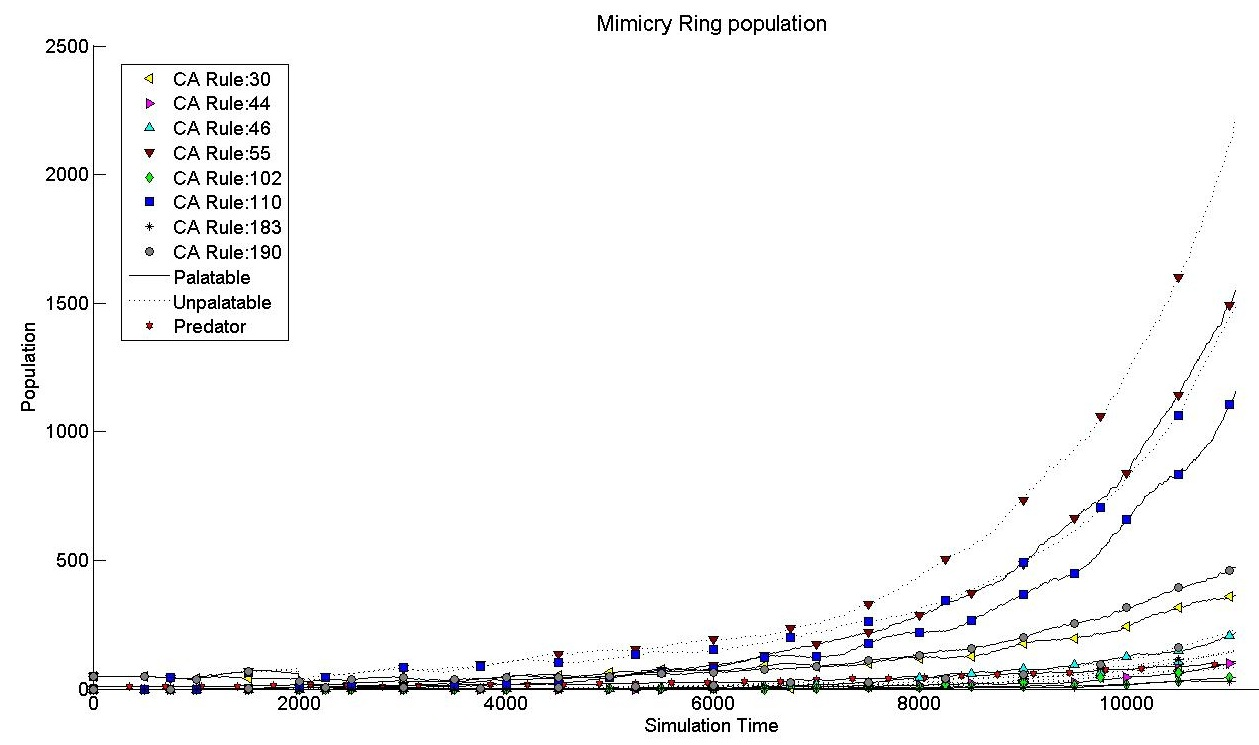
\includegraphics[scale=0.40]{images/simTime10k-4Prey}
	\caption[Population distribution of mimicry rings (4 prey species)]{Population distribution of mimicry rings, initialized with 4 prey species.}
	\label{fig:plot-4-prey}
\end{figure}

By observing the graph in Figure \ref{fig:plot-4-prey} we can see the two rings of unpalatable species which was put at the initial sate of the simulation has dominated after 10000 iterations. CA rule 55 has taken over all other species while CA 110 is following it (represented with dotted curve). Also the palatable prey species with similar patterns to CA rule 55 and 110 are taking full advantage of their deceiving pattern and increasing their population (represented with line curve). The two unpalatable set of patterns CA Rule 90 and 130 are unable to dominate the population. Different other mimicry rings are present in the simulation as we can observe from the graph of number of rings verses simulation time in Figure \ref{fig:ringSize10k-4Prey}, the total number of rings reached somewhere near 33 while each of them has comparatively low representative population. Batesian mimicry is in full effect in this simulated environment.

\begin{figure}[H]
	\centering
	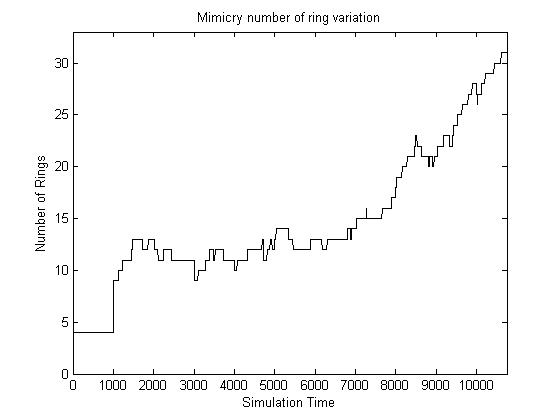
\includegraphics[scale=0.50]{images/ringSize10k-4Prey}
	\caption[Number of mimicry rings (4 prey species)]{Number of mimicry rings, initialized with 4 prey species.}
	\label{fig:ringSize10k-4Prey}
\end{figure}

\begin{figure}[H]
	\centering
	\label{fig:screenshot-simTime11K-4Prey}
	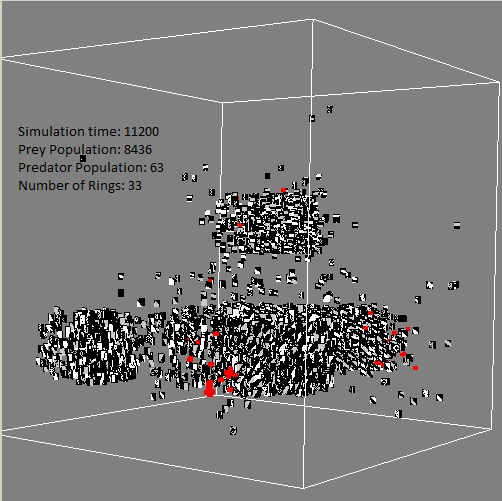
\includegraphics[scale=0.55]{images/simTime11K-4Prey}
	\caption[Graphical representation of the model (simulation time: 11200)]{Graphical representation of the model initialized with 4 prey species, simulation time: 11200.}
\end{figure}

\section{Increased initial population with four prey species}

\begin{table}[H]
\centering
\begin{tabular}{|l|l|c|c|l|c|}
  \hline
   														&\multicolumn{3}{|c|}{Prey configuration} 																	
   														& \multicolumn{2}{|c|}{Predator configuration} \\ \hline
  \multirow{4}{*}{Population} & Rule110 (Palatable) & \parbox[c]{2.1em}{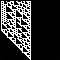
\includegraphics[scale=0.50]{images/CARule110}} & 150 & \multicolumn{2}{|c|}{\multirow{4}{*}{20}} \\ \cline{2-4}
  					 									& Rule30 (Palatable)& \parbox[c]{2.1em}{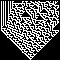
\includegraphics[scale=0.50]{images/CARule30}}  	 & 150 & \multicolumn{2}{|c|}{}\\ \cline{2-4}
  					 									& Rule55 (Unpalatable)& \parbox[c]{2.1em}{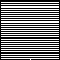
\includegraphics[scale=0.50]{images/CARule55}}  & 150 & \multicolumn{2}{|c|}{}\\ \cline{2-4}
  					 									& Rule190 (Unpalatable)& \parbox[c]{2.1em}{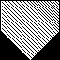
\includegraphics[scale=0.50]{images/CARule190}}& 150 & \multicolumn{2}{|c|}{}\\ \hline
  \multirow{2}{*}{Reproduction} & Age Limit & \multicolumn{2}{|c|}{100}  & \multicolumn{2}{|c|}{500} \\ \cline{2-6}
  						 									& Interval  & \multicolumn{2}{|c|}{1000} & \multicolumn{2}{|c|}{2500} \\ \hline
  \multirow{2}{*}{Mutation Rate} & Pattern   & \multicolumn{2}{|c|}{0.05} & \multicolumn{2}{|c|}{\multirow{2}{*}{0.03}} \\ \cline{2-4}
  						 									 & Genome    & \multicolumn{2}{|c|}{0.5}  & \multicolumn{2}{|c|}{} \\ \hline
  Demise Age	 									 & \multicolumn{3}{|c|}{2000}							& \multicolumn{2}{|c|}{7000} \\ \hline
  Minimum Attack Age						 & \multicolumn{3}{|c|}{} 						    & \multicolumn{2}{|c|}{500} \\ \hline
  \multirow{2}{*}{Memory Configuration} & \multicolumn{3}{|c|}{} 					& Minimum & 4 \\ \cline{5-6}
   																			& \multicolumn{3}{|c|}{} 					& Maximum & 10 \\ \hline  
\end{tabular}
\caption{Agent configuration of 4 prey species with increased population}
\label{tab:config-table-4-more-prey}
\end{table}

In this run of the simulation some significant parameters have been updated. One is the initial population of prey species. It has been increased from 50 to 150 for each of the prey species, while increasing the overall population from 200 to 600. Secondly the number of predator population has been increased from 20 to 30. Thirdly, Predator demise age has been increased from 2500 to 7000 while their reproduction interval has been increased from 1400 to 2500. Increasing predator demise age can have an interesting effect, as the longer a predator is present in a simulation, the longer it will be making intelligent decision in terms of consuming its prey and there will be increased selection pressure from the entire population of predators. 

\begin{figure}[H]
	\centering
	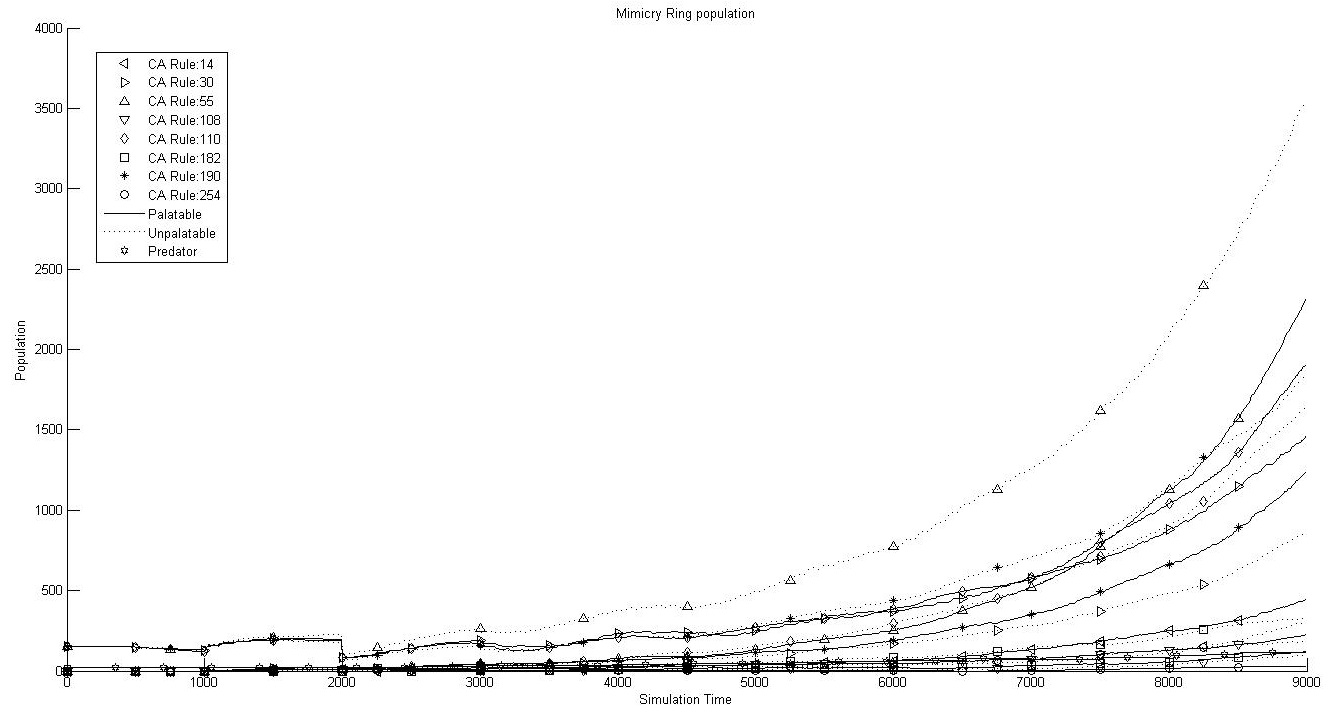
\includegraphics[scale=0.40]{images/simTime9K-4MorePrey}
	\caption[Population distribution of mimicry rings (4 prey species, increased population)]{Population distribution of mimicry rings, initialized with 4 prey species with increased population.}
	\label{fig:plot-4-more-prey}
\end{figure}

Some very interesting diversity of rings can be observed in the simulation for updating these parameters. The unpalatable rings and their deceptive counterparts(palatable prey with similar pattern) still have their dominance. We can observe CA Rule 55 and 190 are the highest number of population. Interestingly enough CA Rule 110 which started as a palatable prey species has also taken dominance in the population which is the second highest. Both palatable and unpalatable version of CA Rule 110 are present with equal population density.

\begin{figure}[H]
	\centering
	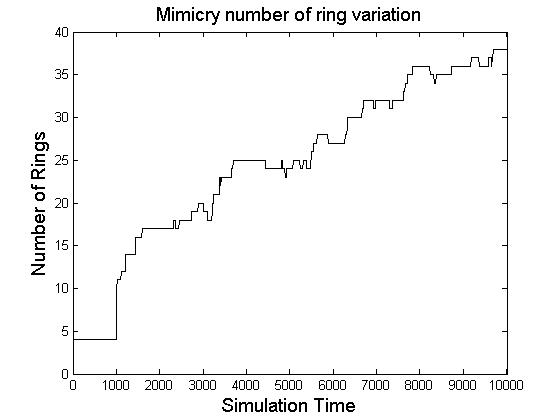
\includegraphics[scale=0.50]{images/ringSize10k-4MorePrey}
	\caption[Number of mimicry rings (4 prey species, increased population)]{Number of mimicry rings, initialized with 4 prey species with increased population.}
	\label{fig:ringSize10k-4MorePrey}
\end{figure}

The total number of rings had much increment in this run compared to the previous one. To summarize we can observe increased diversity of prey population and much more interaction between predators and prey.

\section{Initial population with six prey species}
\begin{table}[H]
\centering
\begin{tabular}{|l|l|c|c|l|c|}
  \hline
   														&\multicolumn{3}{|c|}{Prey configuration} 																	
   														& \multicolumn{2}{|c|}{Predator configuration} \\ \hline
  \multirow{6}{*}{Population} & Rule110 (Palatable) & \parbox[c]{2.1em}{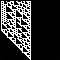
\includegraphics[scale=0.50]{images/CARule110}} 
  																									& 150 & \multicolumn{2}{|c|}{\multirow{6}{*}{30}} \\ \cline{2-4}
  					 									& Rule30  (Unpalatable)& \parbox[c]{2.1em}{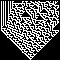
\includegraphics[scale=0.50]{images/CARule30}}  
  					 																				& 150 & \multicolumn{2}{|c|}{}\\ \cline{2-4}
  					 									& Rule55  (Palatable)& \parbox[c]{2.1em}{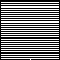
\includegraphics[scale=0.50]{images/CARule55}}    
  					 																				& 150 & \multicolumn{2}{|c|}{}\\ \cline{2-4}
  					 									& Rule190 (Unpalatable)& \parbox[c]{2.1em}{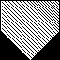
\includegraphics[scale=0.50]{images/CARule190}} 
  					 																				& 150 & \multicolumn{2}{|c|}{}\\ \cline{2-4}
  					 									& Rule57  (Palatable)& \parbox[c]{2.1em}{
\includegraphics[scale=0.50]{images/CARule57}}    
  					 																				& 150 & \multicolumn{2}{|c|}{}\\ \cline{2-4}
  					 									& Rule105 (Unpalatable)& \parbox[c]{2.1em}{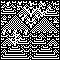
\includegraphics[scale=0.50]{images/CARule105}}& 150 & \multicolumn{2}{|c|}{}\\ \hline
  \multirow{2}{*}{Reproduction} & Age Limit & \multicolumn{2}{|c|}{100}  & \multicolumn{2}{|c|}{500} \\ \cline{2-6}
  						 									& Interval  & \multicolumn{2}{|c|}{1000} & \multicolumn{2}{|c|}{2000} \\ \hline
  \multirow{2}{*}{Mutation Rate} & Pattern   & \multicolumn{2}{|c|}{0.05} & \multicolumn{2}{|c|}{\multirow{2}{*}{0.03}} \\ \cline{2-4}
  						 									 & Genome    & \multicolumn{2}{|c|}{0.5}  & \multicolumn{2}{|c|}{} \\ \hline
  Demise Age	 									 & \multicolumn{3}{|c|}{2000}							& \multicolumn{2}{|c|}{5000} \\ \hline
  Minimum Attack Age						 & \multicolumn{3}{|c|}{} 						    & \multicolumn{2}{|c|}{500} \\ \hline
  \multirow{2}{*}{Memory Configuration} & \multicolumn{3}{|c|}{} 					& Minimum & 6 \\ \cline{5-6}
   																			& \multicolumn{3}{|c|}{} 					& Maximum & 10 \\ \hline  
\end{tabular}
\caption{Agent configuration of 6 prey species.}
\label{tab:config-table-6-prey}
\end{table}

To evaluate the simulation at a more complex level we increase the prey population to 900, consisting of 6 different species with very different pattern configuration. Similarly to increase predator-prey interaction we also increase the number of predator population to 30. Predator reproduction interval has been set comparatively lower in this simulation to 2000 iteration similar to the demise age which is set to 5000. As the initial population of prey species is very high, over time we are expecting even larger number of prey species. If predator population does not increase at similar rate there might be a prey population explosion were predator will have no effect on providing selection pressure for the evolution of mimicry. So that is why predator population control parameter has been set to this level. For memory configuration, the minimum number is set to 6, meaning the predator will have to store 6 different prey pattern configuration before starting to make intelligent decision about consuming them. As previously mention this number is always set in accordance with the initial number of different prey configuration. 

\begin{figure}[H]
	\centering
	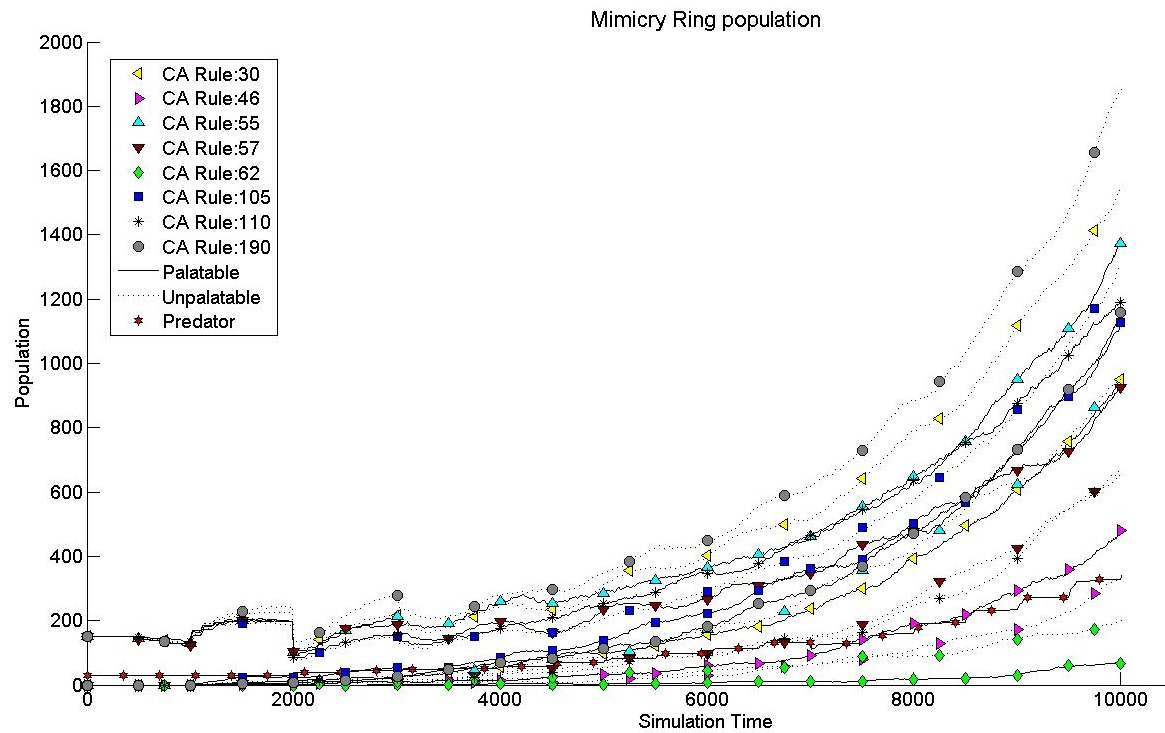
\includegraphics[scale=0.40]{images/simTime10k-6Prey}
	\caption[Population distribution of mimicry rings (6 prey species)]{Population distribution of mimicry rings, initialized with 6 prey species.}
	\label{fig:plot-6-prey}
\end{figure}

With the above set of parameters we can receive the plot of Figure \ref{fig:plot-6-prey}. 

\begin{figure}[H]
	\centering
	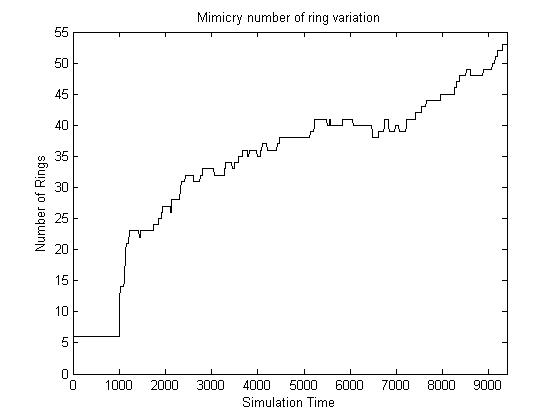
\includegraphics[scale=0.50]{images/ringSize10k-6Prey}
	\caption[Number of mimicry rings (6 prey species)]{Number of mimicry rings, initialized with 6 prey species.}
	\label{fig:ringSize10k-6-Prey}
\end{figure}

\section{Initial configuration with only unpalatable species}
\label{sec:init-conf-only-unp}
\begin{table}[H]
\centering
\begin{tabular}{|l|l|c|c|l|c|}
  \hline
   														&\multicolumn{3}{|c|}{Prey configuration} 																	
   														& \multicolumn{2}{|c|}{Predator configuration} \\ \hline
  \multirow{4}{*}{Population} & Rule110 (Unpalatable) & \parbox[c]{2.1em}{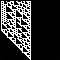
\includegraphics[scale=0.50]{images/CARule110}} 
  																									& 150 & \multicolumn{2}{|c|}{\multirow{4}{*}{30}} \\ \cline{2-4}
  					 									& Rule30  (Unpalatable)& \parbox[c]{2.1em}{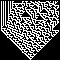
\includegraphics[scale=0.50]{images/CARule30}}  
  					 																				& 150 & \multicolumn{2}{|c|}{}\\ \cline{2-4}
  					 									& Rule55  (Unpalatable)& \parbox[c]{2.1em}{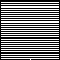
\includegraphics[scale=0.50]{images/CARule55}}    
  					 																				& 150 & \multicolumn{2}{|c|}{}\\ \cline{2-4}
  					 									& Rule190 (Unpalatable)& \parbox[c]{2.1em}{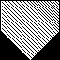
\includegraphics[scale=0.50]{images/CARule190}}& 150 & \multicolumn{2}{|c|}{}\\ \hline
  \multirow{2}{*}{Reproduction} & Age Limit & \multicolumn{2}{|c|}{100}  & \multicolumn{2}{|c|}{500} \\ \cline{2-6}
  						 									& Interval  & \multicolumn{2}{|c|}{1000} & \multicolumn{2}{|c|}{2000} \\ \hline
  \multirow{2}{*}{Mutation Rate} & Pattern   & \multicolumn{2}{|c|}{0.05} & \multicolumn{2}{|c|}{\multirow{2}{*}{0.03}} \\ \cline{2-4}
  						 									 & Genome    & \multicolumn{2}{|c|}{0.5}  & \multicolumn{2}{|c|}{} \\ \hline
  Demise Age	 									 & \multicolumn{3}{|c|}{2000}							& \multicolumn{2}{|c|}{5000} \\ \hline
  Minimum Attack Age						 & \multicolumn{3}{|c|}{} 						    & \multicolumn{2}{|c|}{500} \\ \hline
  \multirow{2}{*}{Memory Configuration} & \multicolumn{3}{|c|}{} 					& Minimum & 4 \\ \cline{5-6}
   																			& \multicolumn{3}{|c|}{} 					& Maximum & 10 \\ \hline  
\end{tabular}
\caption{Agent configuration of 4 prey species all unpalatable.}
\label{tab:config-table-4-prey-unpalatable}
\end{table}

To further observe the effects of mimicry ring we initialize the simulation with four unpalatable population of prey species. As explained earlier the minimum memory configuration is set to 4 as the initial population of prey has four different species. 

\begin{figure}[H]
	\centering
	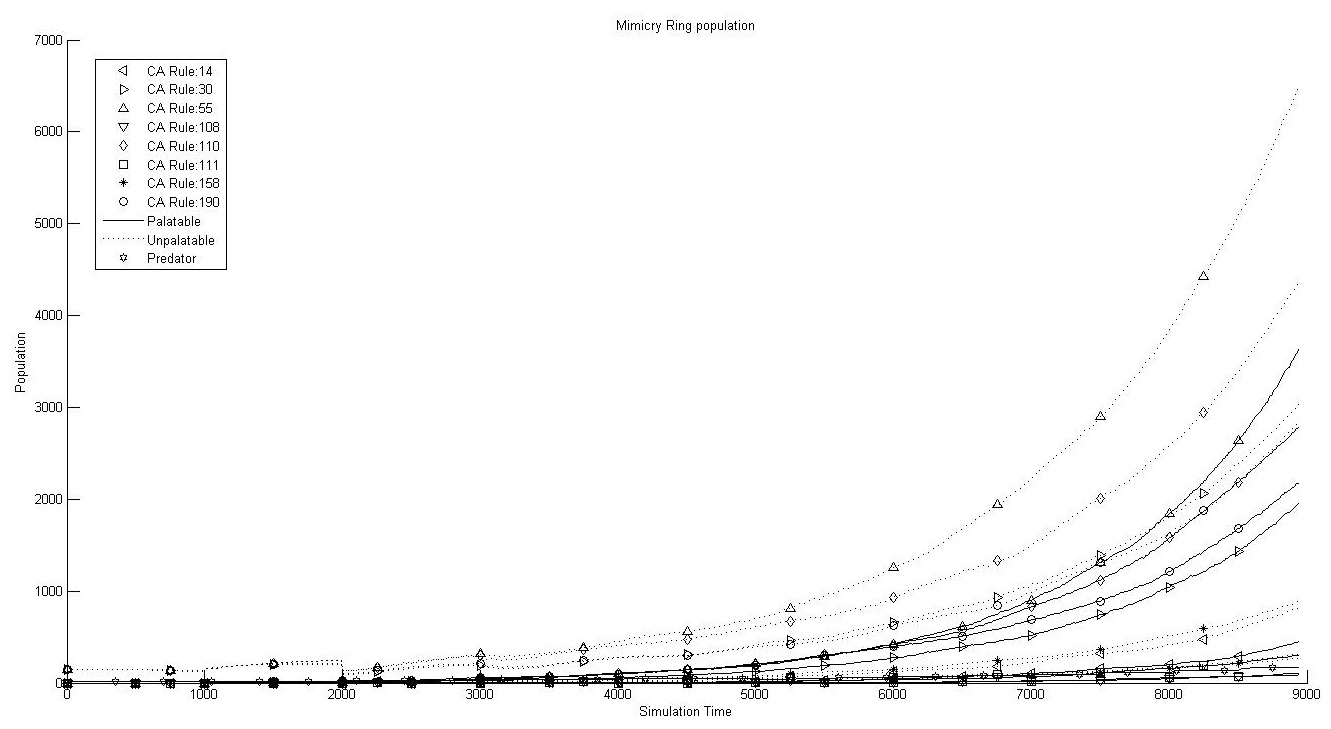
\includegraphics[scale=0.40]{images/simTime-9k-4Prey-unp}
	\caption[Population distribution of mimicry rings(4 prey species all unpalatable)]{Population distribution of mimicry rings, initialized with 4 prey species all unpalatable.}
	\label{fig:plot-4-prey-unp}
\end{figure}

The results according to Figure \ref{fig:plot-4-prey-unp} are expected as it can be observed the population of unpalatable species has prevailed. After nearly 9000 iterations we can see unpalatable species CA rule 55 has prevailed with the most population. Its palatable counter part is following this population. Unpalatable CA Rule 110 and its palatable counter part are also following the above. Similarly the other two species are increasing its population with dominance where the palatable population of deceivers are following them. 

\begin{figure}[H]
	\centering
	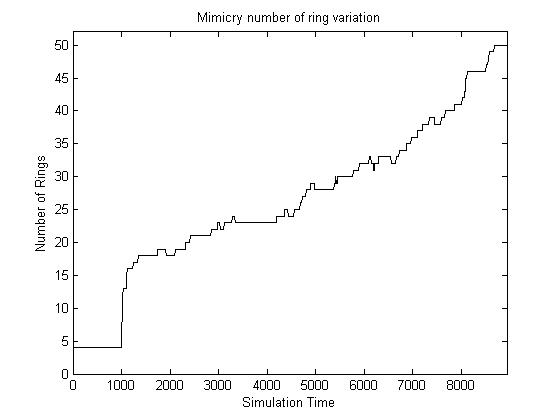
\includegraphics[scale=0.50]{images/ringSize9k-4Prey-unp}
	\caption[Number of mimicry rings (4 prey species all unpalatable)]{Number of mimicry rings, initialized with 4 prey species all unpalatable.}
	\label{fig:ringSize10k-4-Prey-unp}
\end{figure}

\section{Initial configuration with only palatable species}
\label{sec:init-only-palatable-species}

\begin{table}[H]
\centering
\begin{tabular}{|l|l|c|c|l|c|}
  \hline
   														&\multicolumn{3}{|c|}{Prey configuration} 																	
   														& \multicolumn{2}{|c|}{Predator configuration} \\ \hline
  \multirow{4}{*}{Population} & Rule110 (Palatable) & \parbox[c]{2.1em}{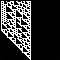
\includegraphics[scale=0.50]{images/CARule110}} 
  																									& 150 & \multicolumn{2}{|c|}{\multirow{4}{*}{30}} \\ \cline{2-4}
  					 									& Rule30  (Palatable)& \parbox[c]{2.1em}{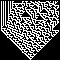
\includegraphics[scale=0.50]{images/CARule30}}  
  					 																				& 150 & \multicolumn{2}{|c|}{}\\ \cline{2-4}
  					 									& Rule55  (Palatable)& \parbox[c]{2.1em}{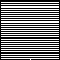
\includegraphics[scale=0.50]{images/CARule55}}    
  					 																				& 150 & \multicolumn{2}{|c|}{}\\ \cline{2-4}
  					 									& Rule190 (Palatable)& \parbox[c]{2.1em}{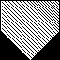
\includegraphics[scale=0.50]{images/CARule190}}& 150 & \multicolumn{2}{|c|}{}\\ \hline
  \multirow{2}{*}{Reproduction} & Age Limit & \multicolumn{2}{|c|}{100}  & \multicolumn{2}{|c|}{500} \\ \cline{2-6}
  						 									& Interval  & \multicolumn{2}{|c|}{1000} & \multicolumn{2}{|c|}{2000} \\ \hline
  \multirow{2}{*}{Mutation Rate} & Pattern   & \multicolumn{2}{|c|}{0.05} & \multicolumn{2}{|c|}{\multirow{2}{*}{0.03}} \\ \cline{2-4}
  						 									 & Genome    & \multicolumn{2}{|c|}{0.5}  & \multicolumn{2}{|c|}{} \\ \hline
  Demise Age	 									 & \multicolumn{3}{|c|}{2000}							& \multicolumn{2}{|c|}{5000} \\ \hline
  Minimum Attack Age						 & \multicolumn{3}{|c|}{} 						    & \multicolumn{2}{|c|}{500} \\ \hline
  \multirow{2}{*}{Memory Configuration} & \multicolumn{3}{|c|}{} 					& Minimum & 4 \\ \cline{5-6}
   																			& \multicolumn{3}{|c|}{} 					& Maximum & 10 \\ \hline  
\end{tabular}
\caption{Agent configuration of 4 prey species all palatable.}
\label{tab:config-table-4-prey-palatable}
\end{table}

The parameters for this simulation has been set exactly the same as in Table \ref{tab:config-table-4-prey-unpalatable} except all the species are palatable at this point. All predator configuration has also been set to exactly same as before.

\begin{figure}[H]
	\centering
	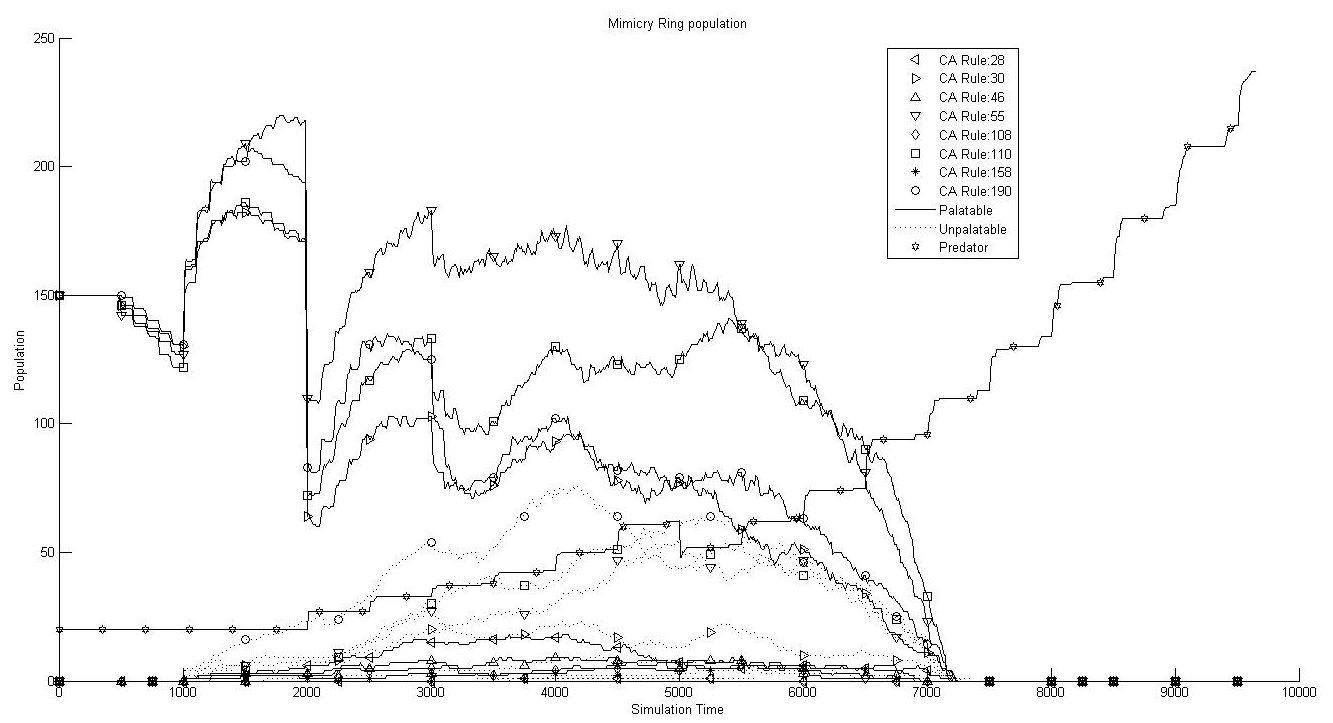
\includegraphics[scale=0.40]{images/simTime-9k-4Prey-p}
	\caption[Population distribution of mimicry rings (4 prey species all palatable)]{Population distribution of mimicry rings, initialized with 4 prey species all palatable.}
	\label{fig:plot-4-prey-p}
\end{figure}

The results for the configuration in Table \ref{tab:config-table-4-prey-palatable} can be observed in Figure \ref{fig:plot-4-prey-p} where all population of prey species have reached its demise at nearly 7000 iterations. By analyzing details we can see, around simulation time 500 all population of species comes to a steady downfall as at this point initial predator species reaches its age for consumption. Around simulation time 1000 all population of prey species start increasing steadily because they reach their maturity level of reproduction. At iteration time 2000 a sudden drop of prey population because the initial population of prey have reached its demise age at this point. By this time the population of unpalatable species deceiving the palatable ones start increasing, and slowly around time 7000 and onwards the entire population of prey comes to its demise. Predator population, from the beginning of the simulation has taken a very dominant effect. As all the species are palatable, predator's consumption and reproduction rate is extremely high and it keeps increasing in a geometric rate.

\begin{figure}[H]
	\centering
	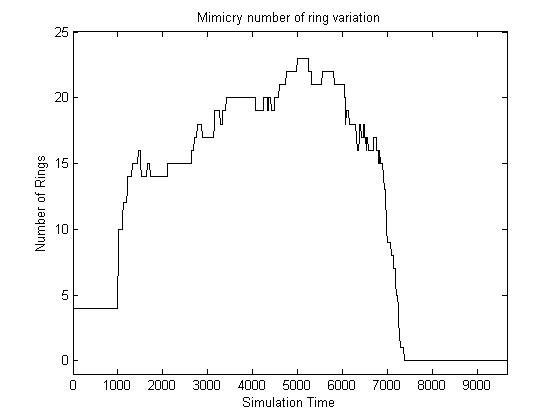
\includegraphics[scale=0.50]{images/ringSize8k-4Prey-p}
	\caption[Number of mimicry rings (4 prey species all palatable)]{Number of mimicry rings, initialized with 4 prey species all palatable.}
	\label{fig:ringSize8k-4-Prey-p}
\end{figure}

Observation of mimicry rings also tell us about the results we have seen in the plot of Figure \ref{fig:plot-4-prey-p}. The number of rings keep increasing but comes to a sudden drop around simulation time 7000 it goes to zero.

\section{Initial configuration with single prey species}
Until now all experiments have been initialized with multiple prey species. The following set of experiments have been done with only a single prey species, for both cases of palatable and unpalatable.

\subsection{Unpalatable}
\label{subsec:single-prey-unpalatable}

\begin{table}[H]
\centering
\begin{tabular}{|l|l|c|c|l|c|}
  \hline
   														&\multicolumn{3}{|c|}{Prey configuration} 																	
   														& \multicolumn{2}{|c|}{Predator configuration} \\ \hline
  Population 									& Rule30 (Unpalatable) & \parbox[c]{2.1em}{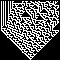
\includegraphics[scale=0.50]{images/CARule30}} 
  																									& 216 & \multicolumn{2}{|c|}{10} \\ \hline
  \multirow{2}{*}{Reproduction} & Age Limit & \multicolumn{2}{|c|}{100}  & \multicolumn{2}{|c|}{500} \\ \cline{2-6}
  						 									& Interval  & \multicolumn{2}{|c|}{1000} & \multicolumn{2}{|c|}{2500} \\ \hline
  \multirow{2}{*}{Mutation Rate} & Pattern   & \multicolumn{2}{|c|}{0.05} & \multicolumn{2}{|c|}{\multirow{2}{*}{0.03}} \\ \cline{2-4}
  						 									 & Genome    & \multicolumn{2}{|c|}{0.5}  & \multicolumn{2}{|c|}{} \\ \hline
  Demise Age	 									 & \multicolumn{3}{|c|}{2000}							& \multicolumn{2}{|c|}{7000} \\ \hline
  Minimum Attack Age						 & \multicolumn{3}{|c|}{} 						    & \multicolumn{2}{|c|}{500} \\ \hline
  \multirow{2}{*}{Memory Configuration} & \multicolumn{3}{|c|}{} 					& Minimum & 2 \\ \cline{5-6}
   																			& \multicolumn{3}{|c|}{} 					& Maximum & 10 \\ \hline  
\end{tabular}
\caption{Agent configuration of 1 prey species unpalatable.}
\label{tab:config-table-1-prey-unpalatable}
\end{table}

This configuration has only one unpalatable species, one in each of the 216 cells, equally distributed all over the environment. Also have a set of 10 predators. Their minimum memory configuration has been set to 2 as any value below 2 will not help the Hopfield Network Memory to differentiate between two patterns.

\begin{figure}[H]
	\centering
	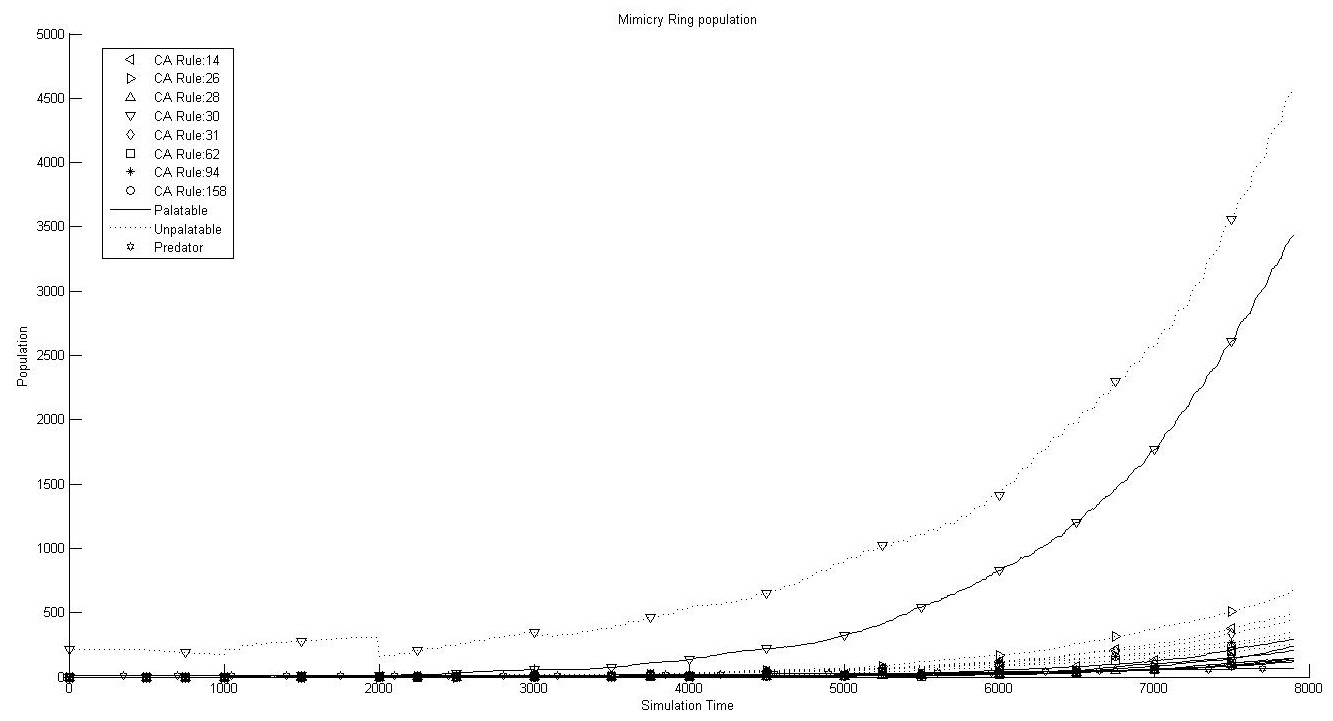
\includegraphics[scale=0.40]{images/simTime8k-1-unp}
	\caption[Population distribution of mimicry rings (1 prey species unpalatable)]{Population distribution of mimicry rings, initialized with 1 prey species unpalatable.}
	\label{fig:plot-1-prey-unp}
\end{figure}

From Figure \ref{fig:plot-1-prey-unp}, it can be observed, the initial set of unpalatable species is dominant as expected. And the palatable population mimicking that set is following it. Also a bunch of other rings with majority of unpalatable species have been created. Mainly because the initial population started with a bunch of unpalatable species, so their evolving generations have similar behavior as well.

\begin{figure}[H]
	\centering
	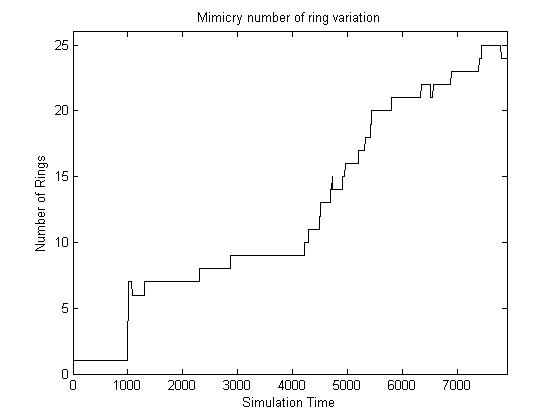
\includegraphics[scale=0.50]{images/ringSize8k-1Prey-unp}
	\caption[Number of mimicry rings (1 prey species unpalatable)]{Number of mimicry rings, initialized with 1 prey species unpalatable.}
	\label{fig:ringSize8k-1-Prey-unp}
\end{figure}

\subsection{Palatable}
\begin{table}[H]
\centering
\begin{tabular}{|l|l|c|c|l|c|}
  \hline
   														&\multicolumn{3}{|c|}{Prey configuration} 																	
   														& \multicolumn{2}{|c|}{Predator configuration} \\ \hline
  Population 									& Rule30 (Palatable) & \parbox[c]{2.1em}{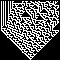
\includegraphics[scale=0.50]{images/CARule30}} 
  																									& 216 & \multicolumn{2}{|c|}{8} \\ \hline
  \multirow{2}{*}{Reproduction} & Age Limit & \multicolumn{2}{|c|}{100}  & \multicolumn{2}{|c|}{500} \\ \cline{2-6}
  						 									& Interval  & \multicolumn{2}{|c|}{1000} & \multicolumn{2}{|c|}{2500} \\ \hline
  \multirow{2}{*}{Mutation Rate} & Pattern   & \multicolumn{2}{|c|}{0.05} & \multicolumn{2}{|c|}{\multirow{2}{*}{0.03}} \\ \cline{2-4}
  						 									 & Genome    & \multicolumn{2}{|c|}{0.5}  & \multicolumn{2}{|c|}{} \\ \hline
  Demise Age	 									 & \multicolumn{3}{|c|}{2000}							& \multicolumn{2}{|c|}{7000} \\ \hline
  Minimum Attack Age						 & \multicolumn{3}{|c|}{} 						    & \multicolumn{2}{|c|}{500} \\ \hline
  \multirow{2}{*}{Memory Configuration} & \multicolumn{3}{|c|}{} 					& Minimum & 2 \\ \cline{5-6}
   																			& \multicolumn{3}{|c|}{} 					& Maximum & 10 \\ \hline  
\end{tabular}
\caption{Agent configuration of 1 prey species palatable.}
\label{tab:config-table-1-prey-palatable}
\end{table}

This configuration is set exactly as according to Section \ref{subsec:single-prey-unpalatable} but with a single set of palatable species. The population of predators have been reduced from 10 to 8 to avoid elimination of all prey species as it happened in case of Section \ref{sec:init-only-palatable-species}.

\begin{figure}[H]
	\centering
	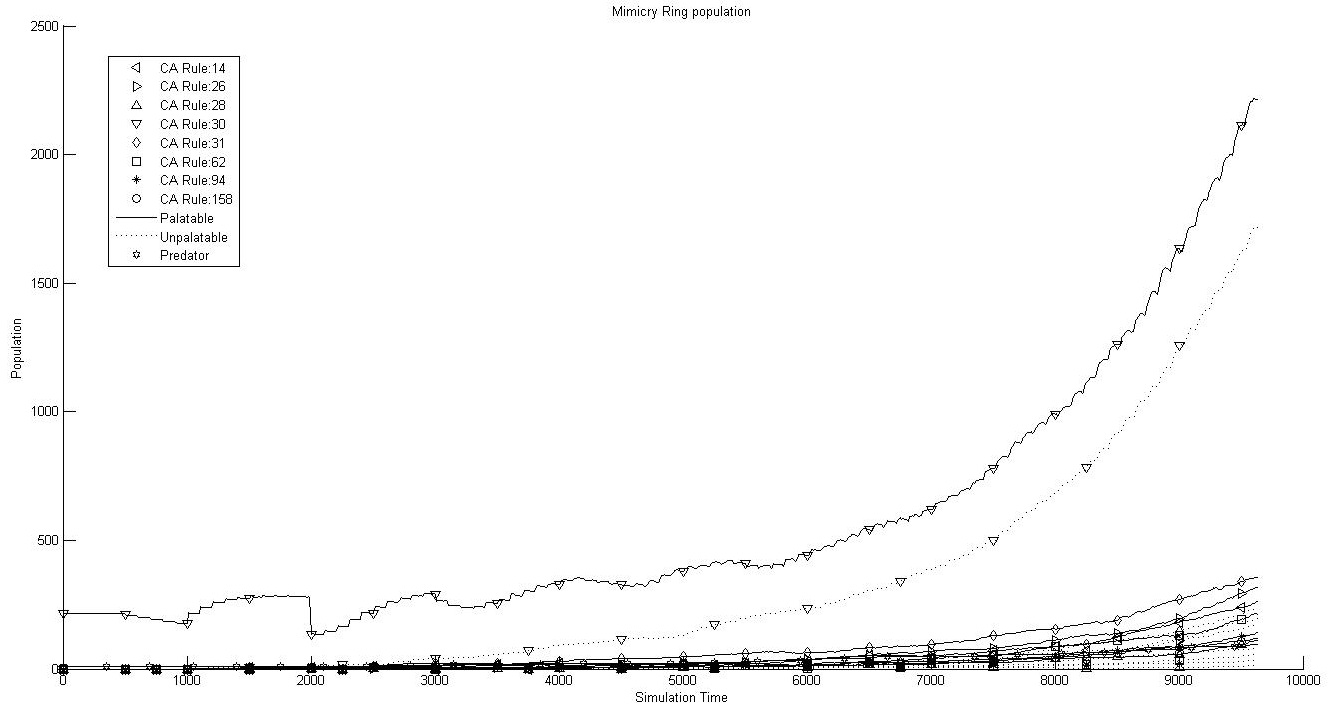
\includegraphics[scale=0.40]{images/simTime9k-1-p}
	\caption[Population distribution of mimicry rings (1 prey species palatable)]{Population distribution of mimicry rings, initialized with 1 prey species palatable.}
	\label{fig:plot-1-prey-p}
\end{figure}

From the initial palatable population we see a bunch of palatable rings created. Major difference from Section \ref{subsec:single-prey-unpalatable} is the total number of prey population created. For the unpalatable species section, total population reaches above 12 thousand. But for palatable species total population reaches nearly above 5000 prey species.

\begin{figure}[H]
	\centering
	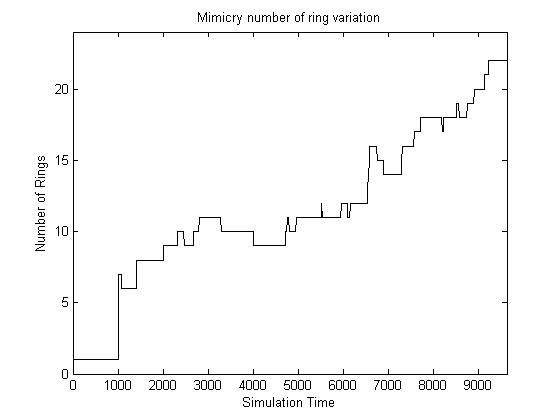
\includegraphics[scale=0.50]{images/ringSize8k-1Prey-p}
	\caption[Number of mimicry rings (1 palatable prey species)]{Number of mimicry rings, initialized with 1 palatable prey species.}
	\label{fig:ringSize8k-1-Prey-p}
\end{figure}

\section{Analysis of Batesian Mimicry}
For all possible initial conditions, Batesian mimicry has taken effect. It can be observed that for every ring of unpalatable species there is an existence of the palatable ring racing to reach the population count of its unpalatable counterpart. Also when the initial population starts with a set of only palatable species we can observe that the total population vanishes within very short period of time (section \ref{sec:init-only-palatable-species}). This effect can be explained with the fact that the palatable population does not have any models to mimic, and it reaches extinction. So from the analysis it can be concluded that the model under discussion has successfully simulated the evolution of Batesian mimicry.

\section{Analysis of Mullerian Mimicry}
Effects of Mullerian mimicry can be observed best for the experiment in section \ref{sec:init-conf-only-unp}. In this experiment we initialize the model with 4 rings of unpalatable species with no palatable ones and after nearly 10K iterations we can observe that all of the initial unpalatable rings have survived with dominance. So we can be conclude that our results match with the one from Frank and Noble (section \ref{subsec:models-by-frank-and-noble}), that multiple Mullerian mimics do not converge into one large ring.

\section{Conclusion}
Analysis of the results tell us that we have successfully been able to simulate the evolution of mimicry. In addition to that, this model provides a more accurate simulation of the fascinating natural process of mimicry rings. Not only does this model simulates mimicry with the initialized population but also it provides possibility of creating diverse new rings and their shift in population. This model also proves the theory of Turner in explaining the evolution of mimicry with punctuated equilibrium (section \ref{subsec:reflection-of-punctuated-equilibrium}) \cite{turner1988}.